\section{Class diagrams}
\todo{needs some explanations}

\subsection{Android}
\subsubsection{The Android view parts}
\begin{figure}[H]
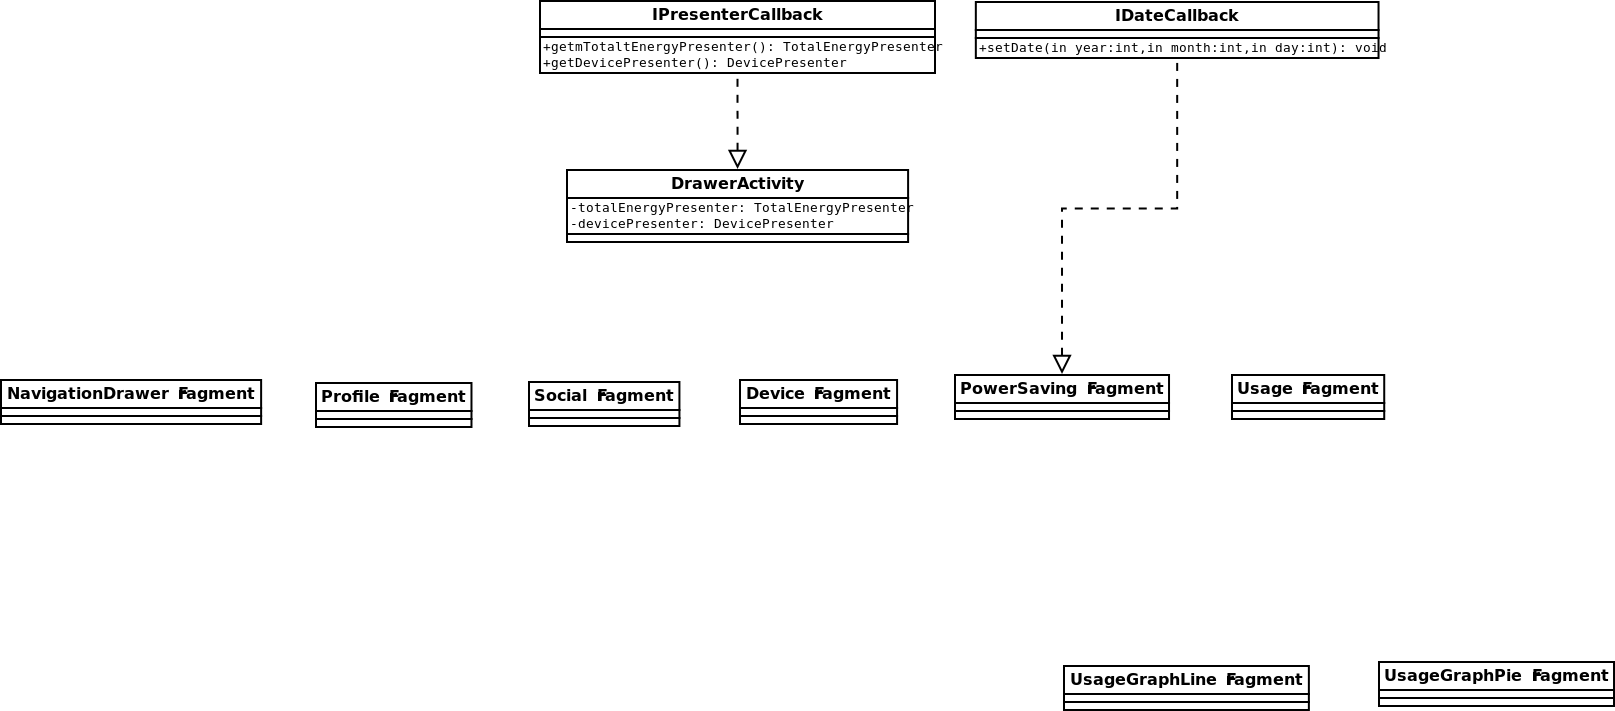
\includegraphics[width=\textwidth]{ch/architecture/fig/ClassDiagramAndroid.png}
\caption{The class diagram for the Android view classes}
\end{figure}

\subsubsection{The Android database part}
\begin{figure}[H]
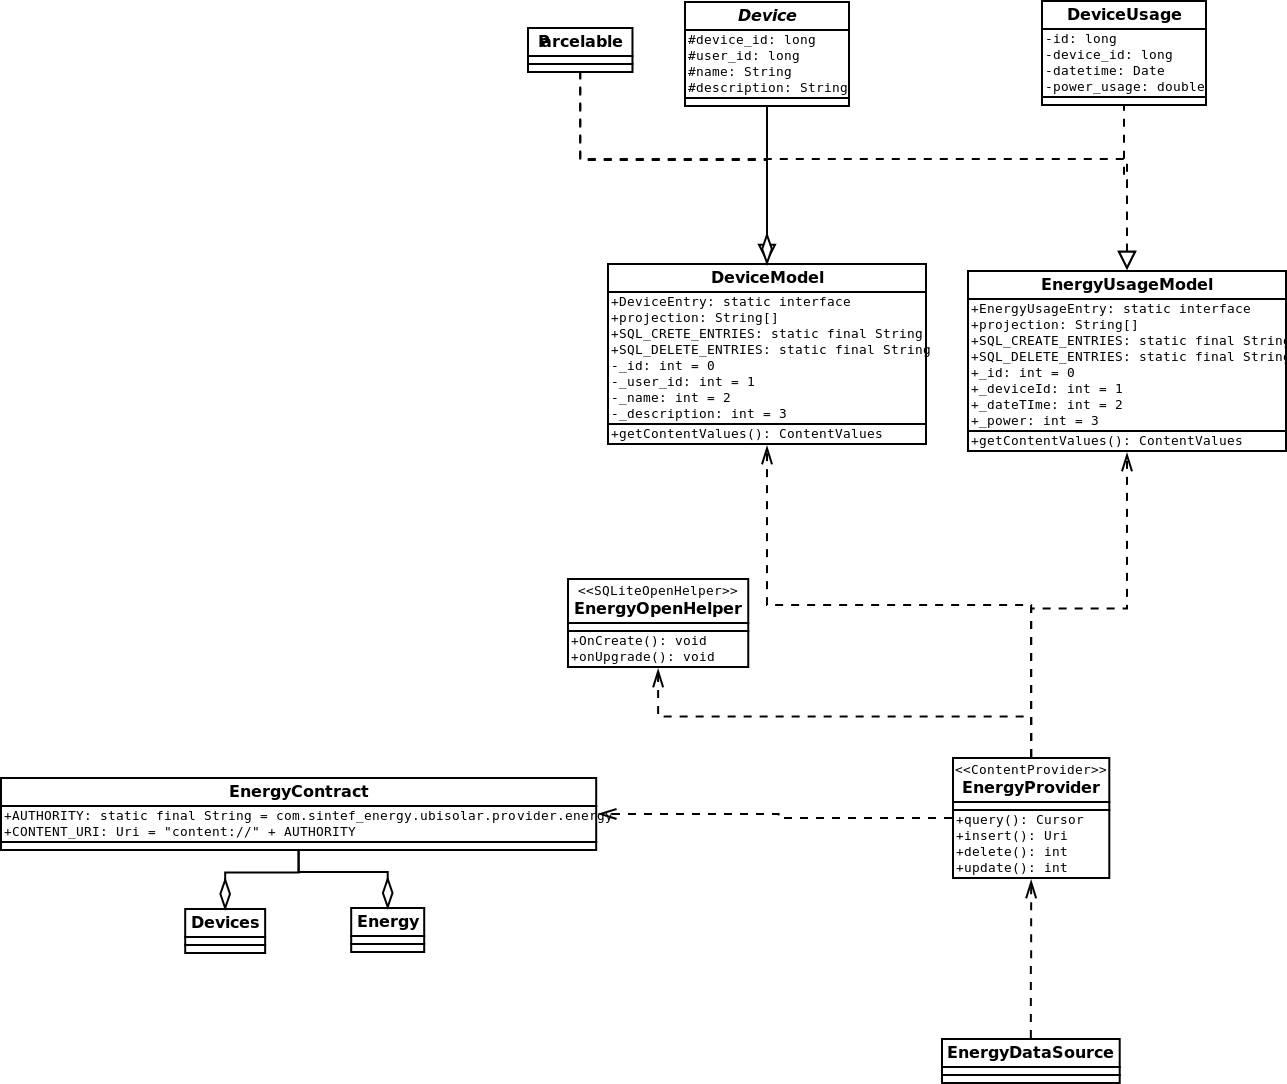
\includegraphics[width=\textwidth]{ch/architecture/fig/classDiagramAndroidDatabase.png}
\caption{Class diagram for the Android database logic}
\end{figure}

\subsubsection{The Android presenter part}

\subsection{Server}
This diagram shows the main structure of how the server uses resources and the database. The main server service creates instances of the resource which when it handles a HTTP request will access the database through the ServerDAO (Server Data Access Object).
\begin{figure}[H]
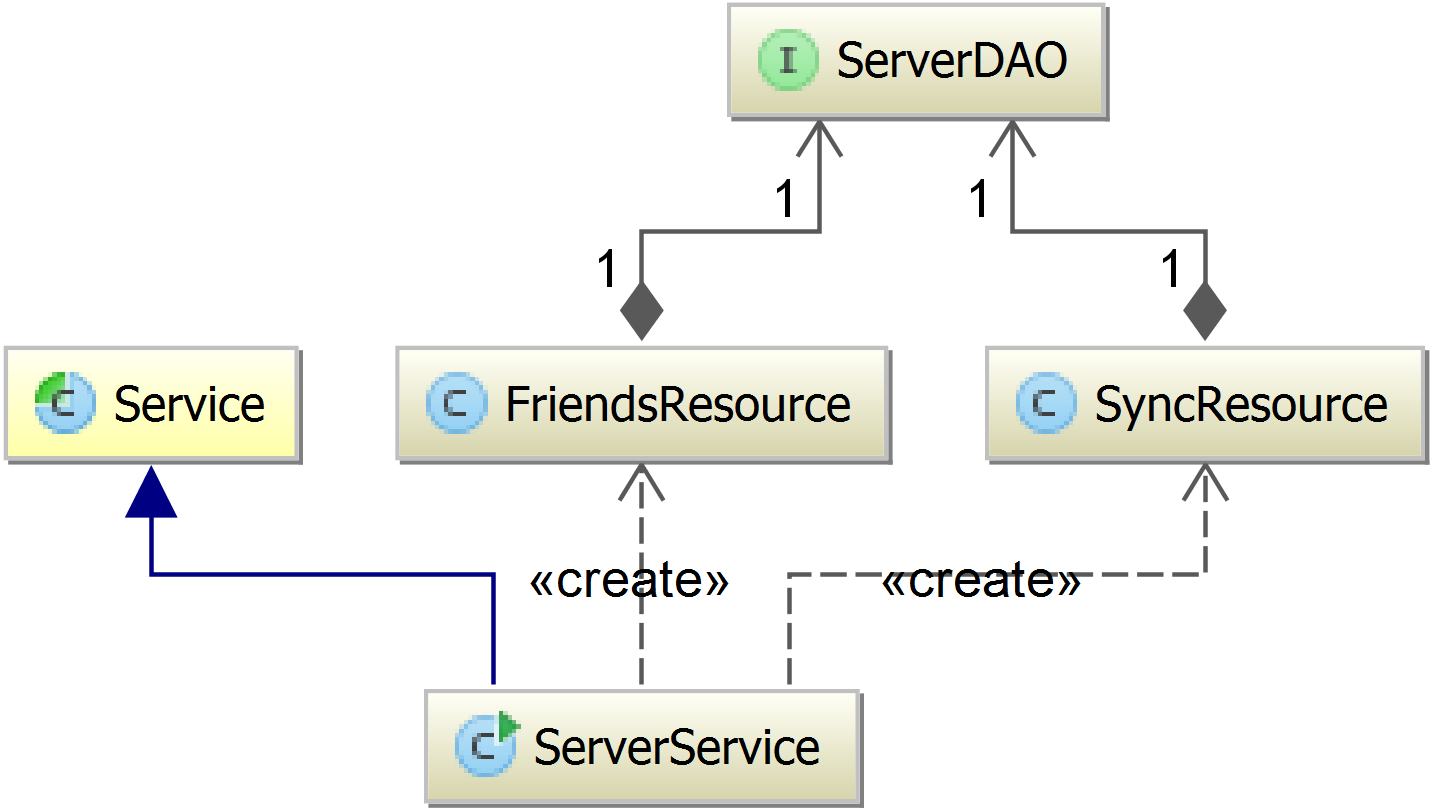
\includegraphics[width=\textwidth]{ch/architecture/fig/classDiagramServer.png}
\caption{Class diagram for main server structure}
\end{figure}

